 \documentclass[a4paper,10pt]{article}
\input{/Users/WannaGetHigh/workspace/latex/macros.tex}

\title{TP 1 : Modification d'images couleur}
\author{Francois \bsc{Lepan}}

\begin{document}
\maketitle

\section{Manipulation de la luminance}

\subsection{D\'ecrire la diff\'erence entre les distributions dans l'espace ad\'equat des couleurs pr\'esentes au sein des images \emph{it1\_72pp} et \emph{it1\_72pp\_sombre}}

\begin{figure}[ht]
\begin{center}
	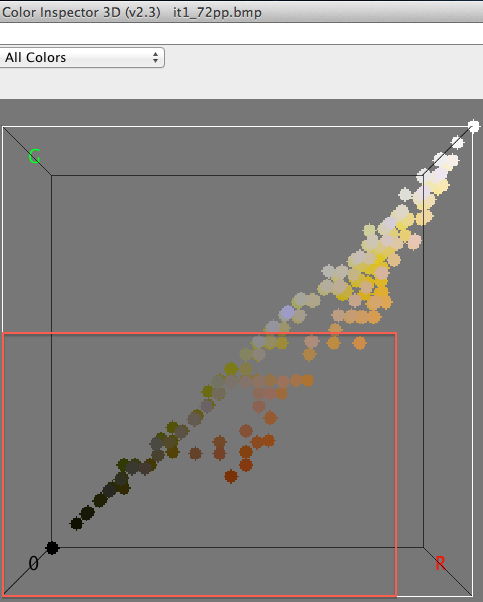
\includegraphics[width=5cm]{images/it1_72pp_inspector}
	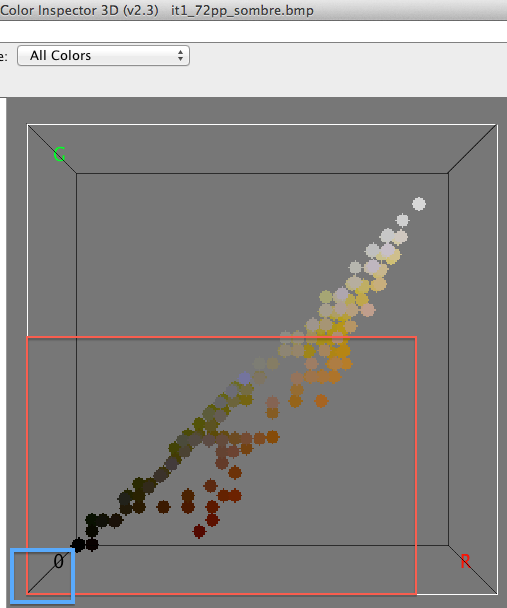
\includegraphics[width=5.2cm]{images/it1_72pp_sombre_inspector}
\end{center}
	\caption{Deux images inspecter via le plugin Color inspector 3D. On retrouve \`a gauche l'image it1\_72\_pp.bmp et \`a droite l'image it1\_72pp\_sombre.bmp}
	\label{img1}
\end{figure}

On remarque sur la ~Fig.~\ref{img1} que la distribution est plus concentr\'e vers le noir (0,0,0) sur l'axe achromatique pour l'image \emph{it1\_72pp\_sombre.bmp}. Ceci est normale vu que cette image est plus sombre que l'image \emph{it1\_72pp.bmp}. Plus pr\'ecis\'ement il y a eu une translation sur l'axe achromatique vers le noir (0,0,0) on voit bien qu'il y a eu une perte d'information entre l'image de gauche et l'image de droite (voir cadre bleu).


\newpage

\subsection{Macro modifiant la luminance}
\begin{Verbatim}[commandchars=\\\{\}]
\codeRed{macro "augmentation_luminance" \{}
image = getImageID();

valeur = getNumber ("quelle augmentation (absolue) de luminance [0-255]",valeur);

while (valeur > 255 && valeur >= 0) \{
	valeur = getNumber ("attention !! juste entre [0-255]",valeur);
\}

setBatchMode(true);

W = getWidth();
H = getHeight();

run("Duplicate...", "title=luminance_augmente_de_"+valeur);
image_luminance_aug = getImageID();

max_1 = 0; 
i_max_1 = 0;
j_max_1 = 0;

for (j=0; j<H; j++) \{
   for (i=0; i<W; i++) \{
	selectImage (image);
	couleur_avant = getPixel(i,j);
	R_avant = (couleur_avant & 0xff0000) >> 16;
	G_avant = (couleur_avant & 0x00ff00) >> 8;
	B_avant = (couleur_avant & 0x0000ff) ;
	
	R_apres = minOf(R_avant + valeur, 255);
	G_apres = minOf(G_avant + valeur, 255);
	B_apres = minOf(B_avant + valeur, 255);

	couleur_apres = ((R_apres & 0xff ) << 16) + ((G_apres & 0xff) << 8) + B_apres & 0xff;


	selectImage (image_luminance_aug);
	setPixel(i,j,couleur_apres);
      	\}
   \}

setBatchMode(false);

\codeRed{\}}
\end{Verbatim}


\subsection{Valeur de $\phi$ qui donne le r\'esultat le plus satisfaisant}

Apr\`es plusieurs essais on trouve que pour une valeur de $\phi$ = 40 l'image r\'esultant est la plus satisfaisante (\emph{cf.} ~Fig.~\ref{it_72pp_changement_luminosite}).

\begin{figure}[ht]
\begin{center}
	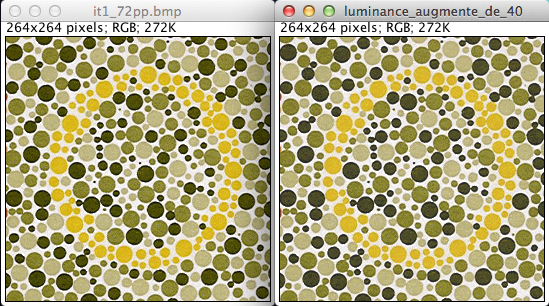
\includegraphics[width=7cm]{images/it_72pp_changement_luminosite.png}
\end{center}
	\caption{\`A gauche l'image \emph{it1\_72pp.bmp} et \`a droite l'image r\'esultante pour $\phi$ = 40}
	\label{it_72pp_changement_luminosite}
\end{figure}

\subsection{Est-ce que l'image r\'esultante est \'egale \`a l'image originale?}

Non car on fait une estimation. Comme expliqu\'e \`a la question 1 on a perdu de l'information donc on ne fait qu'estimer les potentiels valeurs perdu.

\section{R\'etablissement de la saturation}

\subsection{D\'ecrire la diff\'erence entre les distributions dans l'espace ad\'equat des couleurs pr\'esentes au sein des images \emph{it2\_72pp} et \emph{it2\_72pp\_gris}}

\begin{figure}[ht]
\begin{center}
	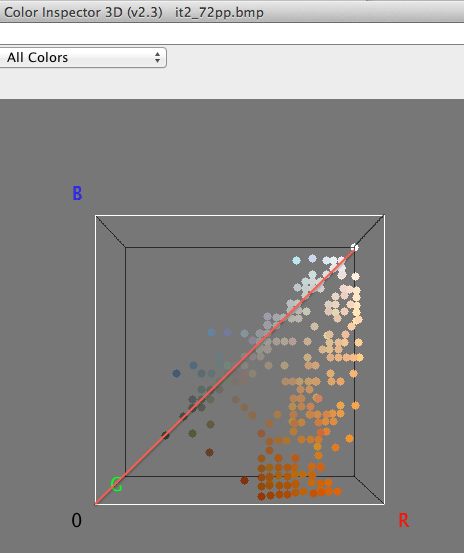
\includegraphics[width=5.2cm]{images/it2_72pp}
	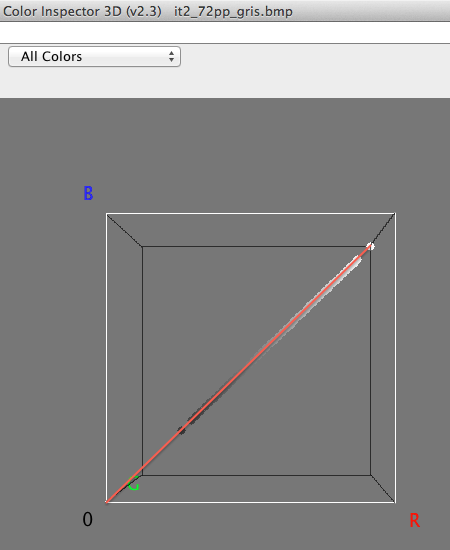
\includegraphics[width=5cm]{images/it2_72pp_gris}
\end{center}
	\caption{Deux images inspecter via le plugin Color inspector 3D. On retrouve \`a gauche l'image it2\_72\_pp.bmp et \`a droite l'image it2\_72pp\_gris.bmp}
	\label{img2}
\end{figure}

On remarque sur la ~Fig.~\ref{img2} que la distribution des couleurs est exclusivement concentr\'e sur l'axe achromatique pour l'image \emph{it2\_72pp\_gris.bmp}.

\subsection{Peut-on \`a partir de \emph{it2\_72pp\_gris} retrouv\'e \emph{it2\_72pp} ?}

Non car on \`a perdu toutes les informations concernant les 3 couleurs RGB pour chaque pixels.

\subsection{D\'ecrire la diff\'erence entre les distributions dans l'espace ad\'equat des couleurs pr\'esentes au sein des images \emph{it2\_72pp} et \emph{it2\_72pp\_saturation}}

\begin{figure}[ht]
\begin{center}
	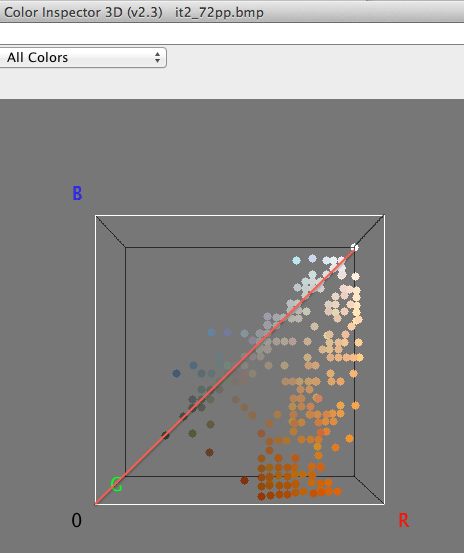
\includegraphics[width=5.25cm]{images/it2_72pp}
	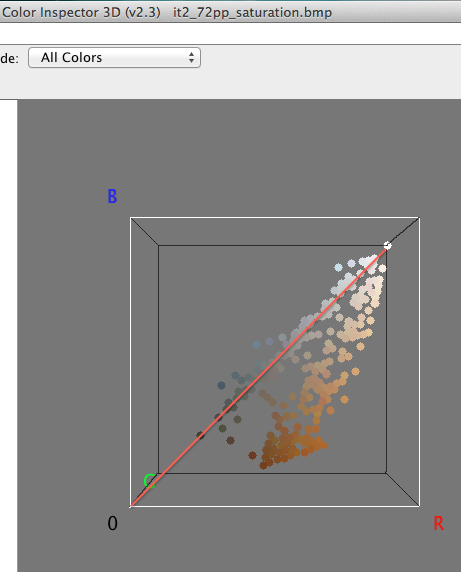
\includegraphics[width=5cm]{images/it2_72pp_saturation}
\end{center}
	\caption{Deux images inspecter via le plugin Color inspector 3D. On retrouve \`a gauche l'image it2\_72\_pp.bmp et \`a droite l'image it2\_72pp\_saturation.bmp}
	\label{img3}
\end{figure}

On remarque sur la ~Fig.~\ref{img3} que la distribution est plus concentr\'e sur l'axe achromatique pour l'image \emph{it2\_72pp\_saturation.bmp}. Il y a juste une diff\'erence d'amplitude, l'image de droite satur\'e a une amplitude de "1" et celle de gauche en poss\`ede une sup\'erieur. La macro suivante nous permettra donc de retrouver la m\^eme image \emph{it2\_72\_pp.bmp} \`a partir de \emph{it2\_72pp\_saturation.bmp}.

\newpage

\subsection{Macro}
\begin{Verbatim}[commandchars=\\\{\}]
\codeRed{macro "changement_saturation" \{}

// recuperation du ID de l'image
image = getImageID();

alpha = getNumber ("quelle valeur pour alpha ? [0-1]",alpha);


while (alpha > 1 || alpha < 0) \{
	alpha = getNumber ("attention !! juste entre [0-1]", alpha);
\}

\codeRed{// on rajoute 1 car on veux augmenter et non abaisser "l'amplitude"}
\codeRed{// des couleurs comme explique dans la question precedente}
alpha += 1;

setBatchMode(true);

W = getWidth();
H = getHeight();

run("Duplicate...", "title= alpha = "+alpha);
image_luminance_aug = getImageID();

for (j=0; j<H; j++) \{
   for (i=0; i<W; i++) \{
	selectImage (image);
	couleur_avant = getPixel(i,j);

	R_avant = (couleur_avant & 0xff0000) >> 16;
	G_avant = (couleur_avant & 0x00ff00) >> 8;
	B_avant = (couleur_avant & 0x0000ff) ;

	Y = (R_avant + G_avant + B_avant)/3;
	
	R_apres = Y + alpha*(R_avant - Y);
        G_apres = Y + alpha*(G_avant - Y);
	B_apres = Y + alpha*(B_avant - Y);

	couleur_apres = ((R_apres & 0xff ) << 16) + ((G_apres & 0xff) << 8) + B_apres & 0xff;

	selectImage (image_luminance_aug);
	setPixel(i,j,couleur_apres);
      	\}
   \}
setBatchMode(false);
\codeRed{\}}
\end{Verbatim}

\subsection{Valeur de $\alpha$ qui donne le r\'esultat le plus satisfaisant}

Apr\`es plusieurs essais on trouve que pour une valeur de $\alpha$ = 1.7.

\subsection{Est-ce que l'image r\'esultante est \'egale \`a l'image originale?}

Oui car la seul diff\'erence entre l'image \emph{it2\_72\_pp.bmp} et \emph{it2\_72pp\_saturation.bmp} est "l'amplitude" des couleurs sur la repr\'esentation 3D. Tout ce que nous avons fait c'est augmenter cette "amplitude".

\section{D\'ecrire la diff\'erence entre les distributions dans l'espace ad\'equat des couleurs pr\'esentes au sein des images \emph{it3\_72pp} et \emph{it3\_72\_sans\_5}}

\begin{figure}[ht]
\begin{center}
	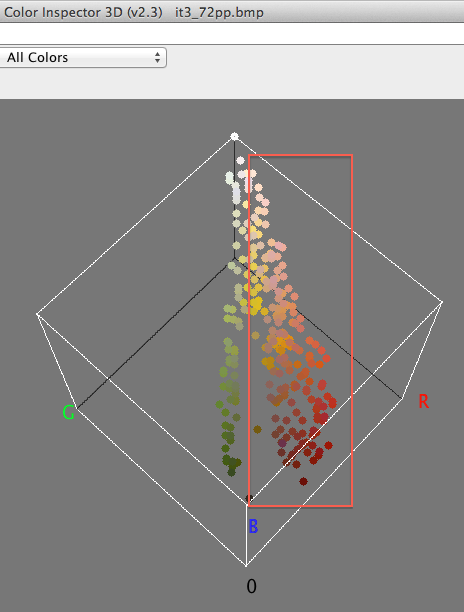
\includegraphics[width=5cm]{images/it3_72pp}
	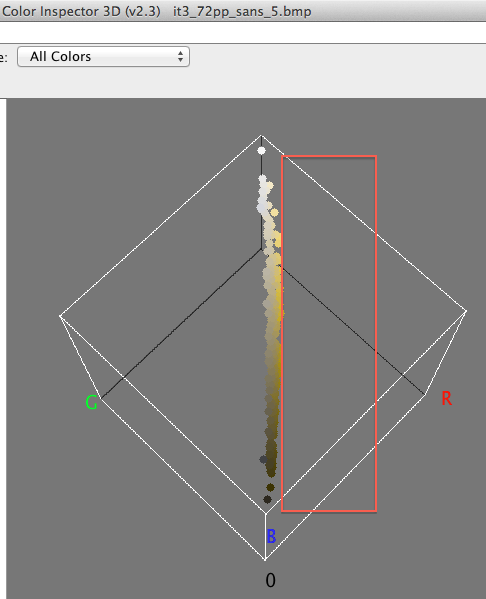
\includegraphics[width=5.3cm]{images/it3_72pp_sans_5}
\end{center}
	\caption{Deux images inspecter via le plugin Color inspector 3D. On retrouve \`a gauche l'image it3\_72\_pp.bmp et \`a droite l'image it3\_72pp\_sans\_5.bmp}
	\label{img4}
\end{figure}

On remarque sur la ~Fig.~\ref{img4} que pour l'image \emph{it3\_72pp\_sans\_5.bmp} il n'y a pas la couleur rouge du 5 dans la distribution des couleurs.

\newpage

\section{D\'ecrire la diff\'erence entre les distributions dans l'espace ad\'equat des couleurs pr\'esentes au sein des images \emph{it1\_72pp} et \emph{it1\_72\_sans\_cercle}}

\begin{figure}[ht]
\begin{center}
	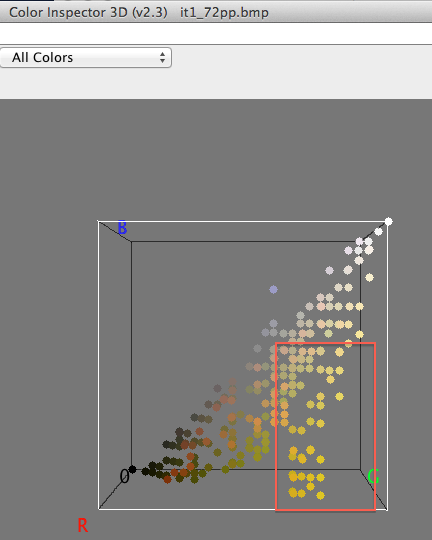
\includegraphics[width=5cm]{images/it1_72pp}
	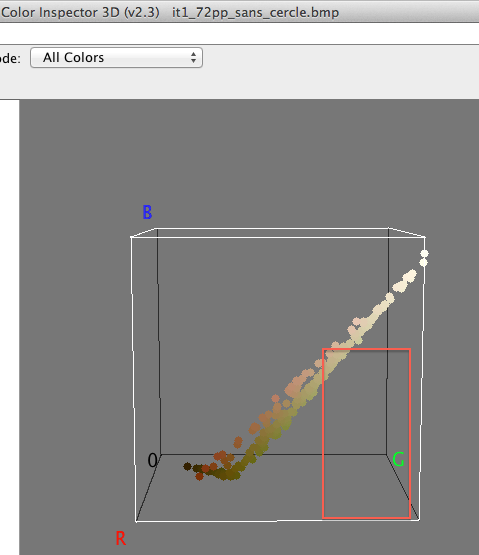
\includegraphics[width=5.3cm]{images/it1_72pp_sans_cercle}
\end{center}
	\caption{Deux images inspecter via le plugin Color inspector 3D. On retrouve \`a gauche l'image it1\_72\_pp.bmp et \`a droite l'image it1\_72pp\_sans\_cercle.bmp}
	\label{img5}
\end{figure}

On remarque sur la ~Fig.~\ref{img5} que pour l'image \emph{it1\_72pp\_sans\_cercle.bmp} il n'y a pas la couleur jaune du cercle dans la distribution des couleurs.


\end{document}